\chapter{Бекаа-82. Часть 1. История.}

\begin{remark}
	 Утром 9 июня 1982 года на всех авиабазах Израиля десятки людей в серо-зеленых несгорающих комбинезонах с окаменевшими лицами повторяют один и тот же полумистический ритуал. Получают боевую задачу. Изучают данные фотосъемки. Согласовывают действия с товарищами, проверяют карты, таблицы связи. Молча вынимают из карманов всё лишнее, что может навредить, если ТАМ что-то пойдёт не так. И снимают погоны, на всякий случай. Каждый хорошо понимает, чем ЭТОТ день может для них закончиться.
	
	Проверяют бомбы, ракеты, топливо, масло, все … Кто-то прячет за привычными действиями нервозность. Кто-то спокоен и сконцентрирован только на цели.
	Запуск двигателя … Последний взгляд – на питание, гидравлику. Повторить «Бадах» (прим. РЛЭ на иврите). Проверить радио. Проверить приборы. Затянуть ремни.
	
	В конце концов, когда кабина захлопывалась, каждый из них остался наедине со своими демонами. Старики, ветераны Войны Судного дня, видели лица своих друзей, однажды взлетевших, но так и не вернувшихся. Молодые – хотели доказать, что они достойны лететь в одном строю со стариками. Кто-то думал о тех, кто остался дома. Кто-то думал о ждущих их сирийских зенитках. Кто-то читал молитву. Как всё пройдёт? До войны в штабе ВВС рассчитали, что на одну батарею придется положить один самолёт. Кто не вернётся на этот раз?
	
	Наконец – взлет. Отпустили тормоза, начали разбег … Ручка чуть вперед, самолет набирает скорость и плавно отрывается от земли. Всё. Ненужные мысли разом улетучились – стало не до них.
	
	Люди в серо-зеленых несгорающих комбинезонах остались один на один со своим вечным врагом.
\end{remark}

В давние времена одному итальянскому генералу пришла в голову идея – если взять тысячу бомбардировщиков, поднять их в воздух и сбросить бомбы на вражеские города, их экономические и логистические центры – враг непременно сдастся, и победа в войне будет неминуема. Звали этого генерала Джулио Дуэ.

В том или ином виде все воюющие страны Второй Мировой пытались воплотить эту идею – сразу, как только научились массово строить бомбардировщики, способные поднять достаточно серьёзную бомбовую нагрузку. У кого-то получалось лучше, кому-то было не до постройки тяжелых четырёхмоторных монстров, но пытались все. И когда первые бомбы упали на землю, встал вопрос -а как с этими монстрами бороться?

Истребители стали вооружаться пушками большего калибра. Появились специализированные войска ПВО, радары, самолеты, предназначенные для перехвата целей на больших высотах. В конце концов, появились целые линии ПВО длиной в десятки километров. А бомбардировщики в ответ стали быстрее, и ощетинились стволами пушек и пулемётов.

В общем, началась борьба между возможностью атаковать и возможностью эту атаку предотвратить.

Первыми и самыми простыми наземными средствами ПВО были зенитные орудия, переделанные из разного рода полевых пушек. Против относительно медлительных машин начала второй большой войны они были достаточно хороши, но с увеличением скорости и высоты бомбардировщика их эффективность падала – при том, что на малых высотах они продолжали быть убийственно эффективными. Требовалось что-то новое.

В пламени конца Второй мировой войны немцы создали новый тип оружия – зенитную ракету. Не от хорошей жизни — они отчаянно искавшие способ борьбы с американскими и английскими «коробками» тяжелых бомбардировщиков, сметавших целые города. А уже после войны этим оружием достаточно быстро обзавелись и американцы, и СССР.

\begin{figure}[h!tb] 
	\centering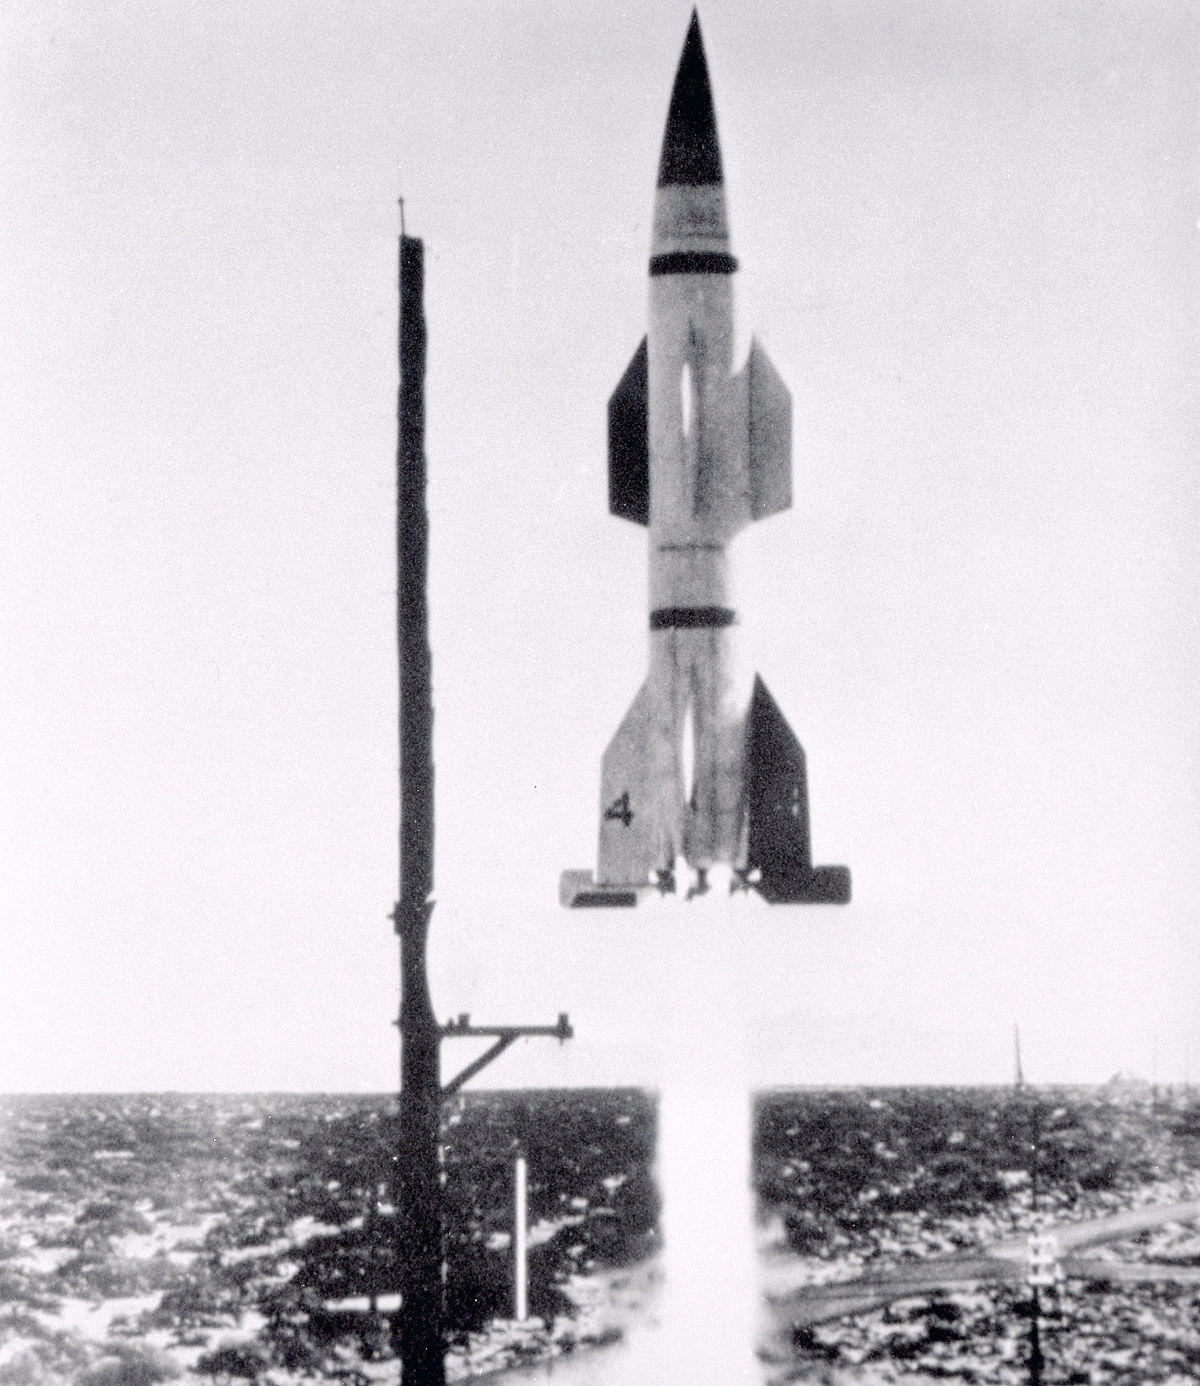
\includegraphics[scale=0.3]{Bekaa_1/zqp4x9QzIUI.jpg}
	%	\label{fig:scipion} % Unique label used for referencing the figure in-text\end{document}
	%	%\addcontentsline{toc}{figure}{Figure \ref{fig:placeholder}} % Uncomment to add the figure to the table of contents%----------------------------------------------------------------------------------------
	\caption{Вассерфаль, первая зенитная ракета (фото-Википедия)}%	CHAPTER 2
\end{figure}

Первые ракеты обладали массой ограничений – на максимальную перегрузку цели, на область применения, и подходили в основном для борьбы с неповоротливыми ядерными бомбовозами. Но постепенно ракеты совершенствовались, и основной их целью становились не проигравшие конкуренцию баллистическим ракетам «стратеги», а новый класс целей – истребитель-бомбардировщик. Быстрый, маневренный, способный уклониться от ракеты и почти моментально изменить высоту полета. Самолёт ушел с больших высот.

С его появлением непосредственно поражение противника осталось основной, но далеко не единственной задачей ЗРК. Наличие ракет ПВО вынуждало авиацию уходить на малые высоты (где вовсю работала ствольная зенитная артиллерия) и сильно снижало точность бомбометания — потому, что летящий в тебя телеграфный столб очень нервирует и отвлекает от основной задачи.

«Большое» противостояние зенитной ракеты и самолета началось во Вьетнаме. Американцы поначалу попытались применить там тактику «больших батальонов» - т.е. действовали крупными группами «Тадов» (F-105) под прикрытием «Фантомов». Проблема была в том, что самолеты у американцев начали неприлично быстро заканчиваться. С этим надо было что-то делать, и в ход пошли различные ухищрения – средства РЭБ, новые тактики, специализированные эскадрильи прорыва ПВО («Дикие ласки»), противорадарные ракеты, и прочее – прочее. Хотя основные потери американцы несли не от ракет, а от все той же TripleA – ствольной артиллерии времен Второй мировой, на малые высоты (на которых AAA наиболее эффективна) американцев загнали как раз ракеты.

\begin{figure}[h!tb] 
	\centering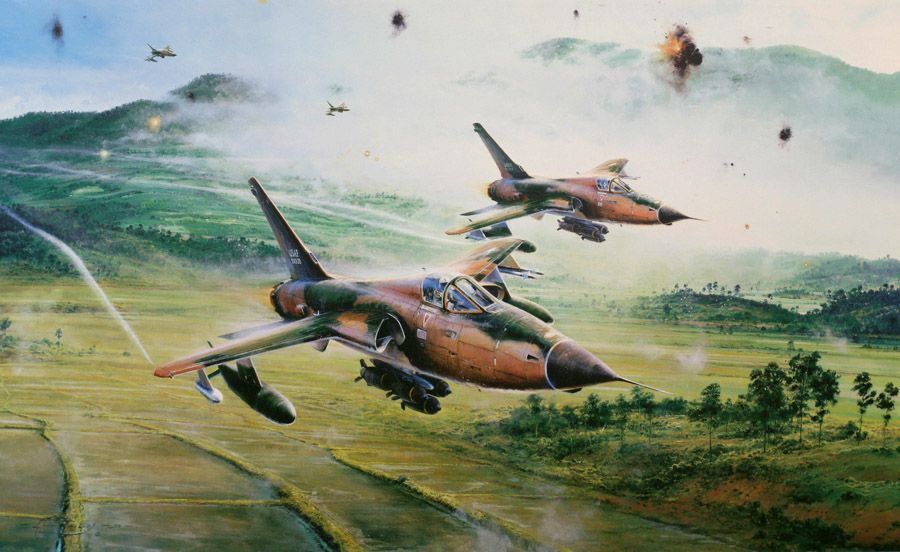
\includegraphics[scale=0.4]{Bekaa_1/nUxQ0UTz6pQ.jpg}
	%	\label{fig:scipion} % Unique label used for referencing the figure in-text\end{document}
	%	%\addcontentsline{toc}{figure}{Figure \ref{fig:placeholder}} % Uncomment to add the figure to the table of contents%----------------------------------------------------------------------------------------
	\caption{F-105 на подходе к цели}%	CHAPTER 2
\end{figure}

Следующий раунд противостояния случился на Ближнем Востоке. В 70-м году прибытие советских «туристов» смогло очень и очень сильно затруднить действия ВВС Израиля – они хоть и потеряли всего 5 самолетов, но операции над Египтом пришлось свести практически к нулю. В 73-м просчеты израильского руководства в начале войны привели к тяжелейшим потерям – за три дня из строя вышли почти 80 (из 400 имевшихся в наличии) самолетов, при этом значительная часть была потеряна безвозвратно. Обстоятельства боев с советскими зенитчиками в 70-м и кошмара 73-го заслуживают отдельного цикла статей, но сейчас речь не об этом.

Война 73-го года отправила командование ВВС Израиля и летчиков в нокдаун. Привычная картина мира (горящие арабские аэродромы, горящие арабские МиГи, горящие арабские задницы) погибла в разрывах ракет «Квадратов» и шквальном огне «Шилок». Некоторые эскадрильи «Скайхоков» и «Фантомов» потеряли до трети самолетов, и их летчики чувствовали себя так, как будто им на голову рухнуло небо. Про небо — это цитата одного из лётчиков.

Здесь надо понимать ещё один момент. Для Израиля (раз уж мы говорим о нем) ВВС – это не просто род войск. Это элита. Это мечта любого подростка. Долгое время их и воспринимали как некую «волшебную палочку», способную решать любую проблему.

Соответственно, до половины оборонного бюджета уходила на летчиков.
Нельзя сказать, что проблемы начала войны 73-го года были внезапны - было несколько достаточно изящных планов уничтожения арабской системы ПВО – предполагалось, что сначала ВВС в течение 1-2 дней расправится с ракетными комплексами, а потом сметет арабские армии на земле. Проблема в том, что этих нескольких дней у них не было – в итоге спасать страну пришлось в условиях противодействия чуть более чем дееспособной ПВО и бардака в штабах с соответствующим результатом.

\begin{figure}[h!tb] 
	\centering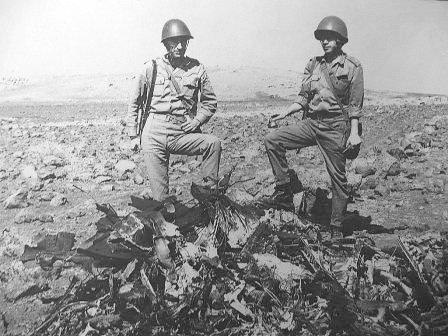
\includegraphics[scale=0.5]{Bekaa_1/Kp2dOPbwwQQ.jpg}
	%	\label{fig:scipion} % Unique label used for referencing the figure in-text\end{document}
	%	%\addcontentsline{toc}{figure}{Figure \ref{fig:placeholder}} % Uncomment to add the figure to the table of contents%----------------------------------------------------------------------------------------
	\caption{Сирийские солдаты фотографируются с результатами плохого планирования}%	CHAPTER 2
\end{figure}

В общем, все то, что произошло в 82-м году – прямое следствие тяжелых потерь Войны Судного дня. Рассматривать события в Ливане в отрыве от тяжелых потерь первых дней Войны Судного – примерно то же, что рассматривать причины Второй мировой войны в отрыве от Первой.

Уже после 74-го начались серьезные структурные изменения. Из тех, которые касались именно задач SEAD (т.е. подавления ПВО), можно отметить следующие:

\begin{itemize}
	\item Реорганизация разведки ВВС. Фактически, уже с 74-го года было понимание, что нужно стремиться к работе «в режиме реального времени». Из него вытекал следующий пункт

\item Увеличение роли беспилотной авиации – фактически, существенную долю задач разведки перенесли на БПЛА – в основном наиболее опасную. Мне несколько раз встречалась информация о том, что в 82-м году беспилотники использовались также в качестве носителя средств РЭБ/РТР, но с уверенностью об этом говорить сложно. Технически такая возможность вполне существовала.

\item Огромное количество новых разработок в области радиоэлектронной борьбы. Возможности ВВС в 73-м и 82-м отличались как два разных мира. Можно уверенно сказать, что это была наиболее эволюционировавшая с 73-го года область.

\item Подготовка летчиков. После 73-го года «фокус внимания» ВВС окончательно переместился с небес на землю. Для многих летчиков «поколения Войны Судного дня» основной целью было сбить вражеский самолет. Отбомбиться – да, хорошо, но «задачей для настоящих мужчин» считался именно воздушный бой. После 73-го года такое восприятие начало меняться.

Отбор на летный курс существенно ужесточили. Хотя, казалось бы, куда еще дальше? Искали наиболее психологически устойчивых и твердых кандидатов. Некоторый комизм был в том, что многие молодые израильтяне, не прошедшие отбор в летный состав, уходили служить в различный спецназ, столь высоки были требования к летчикам.

\item Появление нового, управляемого оружия.

\item Обучение борьбы с ЗРК на всех этапах подготовки летчика – в летной школе, на курсах боевого применения, в эскадрилье. Многие из тех задач, которые стали «классическими» для послевоенного поколения, до 73-го года были второстепенными. Например — защита собственных аэродромов.
Для имитации арабских ЗРК было создано целое наземное подразделение и несколько специальных «площадок» в пустыне Негев. Важно было научиться работать в режиме реального времени, и научиться можно было только на «живом» примере. 
\end{itemize}

Классическим способом преодоления ПВО того времени была отправка достаточно большого количества самолетов с неуправляемым бомбами и противорадарными ракетами. Сам этот способ порождал несколько проблем:
\begin{enumerate}
	\item Разведка. Обнаружение позиций ЗРК возможно двумя основными способами – при помощи авиаразведки (более точное) и средств радиотехнической разведки (менее точное). В обоих случаях, аппарат, проводящий разведку, подвергается существенной опасности.
	\item Подход к цели. Выход к цели на больших высотах подставляет ударную группу под ракеты ПВО и лишает фактора внезапности, на малых высотах – группа попадает под огонь ПЗРК и ствольной артиллерии.
	\item Подтверждение успешности атаки. Для того, чтобы гарантированно уничтожить цель, нужно было отправить не одно, а 2-3 звена, что существенно увеличивало нагрузку на ударную авиацию.
\end{enumerate}

Именно возможность перераспределять задачи ударных звеньев непосредственно в воздухе стали одной из главных «фишек» израильтян в 82 году – фактически, благодаря беспилотникам с телекамерами, за действиями ударной авиации стало возможно наблюдать «в режиме реального времени» - с точки зрения управления авиацией это было настоящей революцией. Это не избавляло от неразберихи целиком и полностью, но существенно повышало эффективность.

Другой революцией были средства РЭБ – в Войну Судного дня они были представлены главным образом наземными станциями и вертолетами постановки помех («Катеф»), а те же диполи нередко возили в воздушных тормозах. В 82-м году все это казалось смешной архаикой – ВВС обзавелись специализированными самолетами (на базе 707 Боинга и «Аравы»), вертолетами, подвесными контейнерами и кучей других вещей, многие из которых до сих пор неизвестны. В итоге, они просто парализовали работу наземных и авиационных РЛС сирийцев.

И это только самое важное – появились управляемые бомбы, новые ракеты, и огромное множество других интересных штук. Как правило – американского производства, но существенно доработанных в самом Израиле. Почему доработанных? «Из коробки» с точки зрения израильтян они были весьма паршивы, а после своего рода «напилинга» – ничего, можно успешно воевать. Одним из ярких примеров такого рода доработок были новые «Маверики» и проект Purple fist. В общем, в течение 9 лет огромное количество людей в ВВС было одержимо идеей реванша за 73-й год. Мало кто сомневался, что такой случай представится. В итоге, так и получилось.

Иногда говорят, что в основе каждой большой победы лежит болезненное поражение. Бекаа-82 - не исключение. Сегодня мы поговорим об одном таком.

Многие люди по неизвестной мне причине пребывают в уверенности, что евреи всегда побеждали арабов. Легко и непринужденно. “Арабы не вояки” говорят они. Мне всегда казалось, что Гиват-ха-Тахмошет, Карамэ, Китайская ферма и Долина слез, доказали обратное. Но нет. Приведем еще один пример.

7 июня 1973 года, на второй день Войны Судного дня, примерно 40 экипажей смешанной ударной группы трех израильских эскадрилий “Фантомов” (201, 69 и 107й) подняли в воздух свои самолеты. Задача казалась простой - избавиться от нескольких батарей сирийских “Квадратов”, осложняющих жизнь израильским штурмовикам - “Скайхокам” на Голанах.

План был такой - на малых высотах подойти к батареям, набрать высоту, обнаружить позиции ЗРК, отбомбиться и уйти. Но, как водится, гладко было на бумаге. Из-за тотального бардака начала войны, вертолеты РЭБ остались на Синае, а эскадрилью ложных целей - беспилотников просто забыли (!) предупредить об изменившемся времени атаки - в итоге они отстрелялись в никуда. Для полного счастья, маршрут ударных групп пролегал через узел сирийской ствольной ПВО одной из бронетанковых дивизий.

Но самое главное выяснилось уже на месте. Израильские пилоты с удивлением обнаружили, что предполагаемые позиции батарей ЗРК просто - напросто ПУСТЫ. Да, за ночь мобильные “Квадраты” сумели переместиться существенно ближе к линии фронта.

Операция закончилась катастрофой. Два “Фантома” были сбиты на подходе к цели. Два - над целью. Два - при отходе от цели. Что характерно, все - “Шилками” или ствольной артиллерией. Ситуация в какой-то момент стала настолько критической, что один из штурманов “Фантома” просто катапультировал себя при близком разрыве ракеты - что характерно, пилот довел поврежденный самолет на аэродром. Через 10 дней он погиб на Синае - возможно, штурману стоило катапультировать их обоих.

Шесть “Фантомов” превратились в факелы на земле. Десять других - тяжело повреждены и не могут лететь. Еще дюжина - быстро вернулась в строй. Девять человек, летчики и штурманы, меняют офицерское общежитие на карцер сирийской тюрьмы.

Двое, лучшие из лучших, погибли.

Результат операции? Выведен из строя один (!) дивизион С-75.
Провал? Провал. Как так получилось?

Ответ просто - операцию просто-напросто чудовищно плохо спланировали. Впопыхах и на фоне зарождающейся паники на самом верху системы принятия решений. Начавшиеся в процессе выполнения проблемы только усугубили ситуацию. Первая волна “Фантомов” пошла, не попала, потому что целевой батареи не было на месте, а данные фоторазведки просто отсутствовали. В итоге один не попал, другого сбили по дороге, а третий сбросил бомбы не туда, потому что думал не так, как надо было. И так далее.

Проблемы были во всем - начиная с разведки (в день операции стояла низкая облачность - при подготовке маршрутов руководствовались фотосъемкой предыдущего дня), и заканчивая отказом отдать инициативу в планировании в эскадрильи. Штаб ВВС отступил от привычного подхода “с нас задача - с вас решение” в пользу «я начальник, я так вижу». Результат не замедлил проявиться.

Собственно говоря, провал этой операции (называлась они “Дугман-5”) и лег в основу многих из тех процессов, которые привели к реформам и грандиозному успеху 82-го года. Если бы тот налет удался - возможно, ВВС почивали бы на лаврах еще довольно долго.

Кстати. А как вообще в те времена боролись с ЗРК?

С того момента как американцы во Вьетнаме поняли, что ракеты создают слишком много проблем, они начали придумывать средства борьбы с ними. В ход пошли разные тактические ухищрения, специализированные эскадрильи борьбы с ЗРК, средства РЭБ и так далее. И вся эта война становилась все хитрее и хитрее.

Так сложилось, что в разработке ЗРК лидировал СССР, а в авиации лидировали США. Не всегда, не везде (в СССР, например, была масса весьма совершенных авиационных средств РЭБ и отличных самолетов), но в большинстве ситуаций это было верно.

Собственно, подход к уничтожению ПВО в 70-х выглядел следующим образом: 
\begin{enumerate}
	\item Обнаружить местонахождения комплекса и идентифицировать его. Как правило, эту задачу возлагали на самолеты фоторазведки и чуть позже – на беспилотники и средства РТР.
	\item Атаковать цель – одним или несколькими звеньями истребителей-бомбардировщиков.
	\item Подтвердить результат атаки средствами из п.1, при необходимости повторить.
\end{enumerate}

Понятно, что противник - не дурак, что свои батареи ЗРК в такой ситуации он будет всячески защищать – в ход пойдет зенитная артиллерия, расчеты ПЗРК, оборудованные ложные позиции, и так далее. Вообще ЗРК (и пусковые, и станции наведения) найти не всегда просто - он, зараза такая, часто не излучает и может быть хорошо спрятан.

Вообще, у защищающейся стороны в такой ситуации есть только одна проблема – инициатива будет гарантированно на стороне противника – именно он будет решать, где и когда нанести удар. Это заставляет обороняющихся держать существенный наряд сил в постоянной боевой готовности, что в целом тоже не здорово.

А дальше начинаются чистой воды шахматы. Потому что, еще раз, бойцы ПВО не будут ждать, когда к ним прилетит волшебник в самолете с пятиконечной (или шестиконечной) звездой и кинет на них бомбу. Противник тоже жить хочет и будет всячески мешать себя уничтожить.

Задача авиации – прорваться к ЗРК/охраняемому объекту и уничтожить их. Задача ПВО – не дать им этого сделать, и по возможности – сбить атакующего.

В начале 70-х было два основных подхода – или работать на малых высотах, пользуясь внезапностью, или на средних, под прикрытием помех. Оба способа имели свои плюсы и минусы.

Главный плюс малых высот – внезапность удара и малое время нахождения в зоне поражения. Минус – самолет на таких высотах представляет собой фантастически хорошую цель для ствольной зенитной артиллерии.

На бОльших высотах все несколько иначе. Самолет недосягаем для эффективного огня орудий ПВО с земли – но представляет собой отличную цель для ракет. Можно надеяться на средства РЭБ и зенитные маневры – но будут ли они эффективны.

До начала Войны Судного дня основным способом атаки позиций ПВО был подход на малых высотах с последующим ударом с кабрирования (методы «Кела» и «Хатаф»). «Шилки» и ЗСУ 2-23 внесли большие коррективы в этот план. Стало понятно, что малые высоты стали смертельно опасными для ударной авиации. Средние и большие высоты уверенно перекрывались ЗРК – «Квадратами», С-75 и С-125, огромное количество которых было поставлено арабам Советским Союзом.

Проблема? Проблема.

Во время Войны Судного дня израильтяне для ее решения часто применяли сложные и смешанные тактики – часть самолетов демонстративной группы постоянно держала расчеты арабских ЗРК в постоянной готовности, часть – блокировала аэродромы истребителей. Первая волна самолетов с кабрирования бомбила позиции ствольной артиллерии, чтобы заставить их расчеты «пригнуть головы» и дать возможность второй волне прорваться к цели. Тут в ход шли противорадарные ракеты, кластерные бомбы и прочие средства уничтожения себе подобных.
Получалось очень так себе.

Кстати о противорадарных ракетах. Вопреки расхожему мнению, их основной целью являлось не столько поражение постов РЛС, сколько отвлечение их расчетов на собственное выживание. Расчет станции наведения ЗРК тоже хочет жить, когда в него летит ракета - и часто выключает радар. Или использует иные способы противодействия.

Короче, на каждое действие есть свое противодействие. Как я уже писал, после Войны Судного дня, в которой израильтяне понесли большие потери от действий ЗРК, стало понятно, что подходе к борьбе с ПВО надо менять – потому что еще одной такой войны ВВС могут не потянуть - а тысяч самолетов, как у американцев, у них нет.

В 74-м разобрались в произошедшем. В 75-м начали думать, что делать. Выводы весьма и весьма делают честь израильтянам. Они в итоге пришли к одному очень грамотному выводу.

При помощи отдельных, даже самых совершенных средств, войну не выиграть. При помощи одних только новых тактик - тоже. Управляемые бомбы, ракеты, подвесные контейнеры - все они не гарантируют победы. Новые самолеты, сколько угодно хорошие, при бездарном применении - просто мишень (иранцы и саудиты это уверенно доказали и не собираются останавливаться).

Ты можешь обладать лучшими платформами - но для победы нужна интеграция всех систем в одну. Потому что только когда подготовленные пилоты получат новое оружие, новые самолеты, когда наводить их на цель будут в режиме реального времени - тогда они будут практически непобедимы.

В общем, со скучной но необходимой теорией на сегодня закончили пора поговорить о заклятых друзьях израильтян - сирийцах. О том, как они собирались воевать. И об одном фундаментальном различии между ними и израильтянами - возможно, самом важном и определяющим.

До этого момента мы говорили в основном об Израиле и авиации - но рассказ об арабо-израильских войнах без подробного упоминания арабов это как свадьба без невесты - или немного странно, или вообще противоестественно. Или как реконструкция Второй мировой без немцев, тоже то еще извращение.

Я не хочу вдаваться в детальное описание каждого комплекса, стоявшего на вооружении сирийской армии - я в первую очередь хочу описать несколько основных закономерностей, с ней связанных.

Во-первых, сирийская армия (и в особенности - авиация и ПВО) комплектовались достаточно разнородными по стране - производителю комплексами, что отличало ее, например, от советской армии. Ещё её отличало то, что комплектовалась она отборными арабами, но это частности. Например, на вооружении сирийцев Ми-24 (не успели повоевать в Ливане) успешно соседствовали с франуцзскими “Газелями”, которые ухитрились стать наиболее “проблемным” для израильтян сирийским летательным аппаратом в той войне. Инструктора в Сирии тоже были из разных стран, в основном социалистических, не только из СССР.

Во-вторых, Союз как правило не поставлял арабам самую современную технику. Надо сказать, что американцы тоже не рвались давать Израилю лучшее оружие. Проблема в том, что израильтяне придумали достаточно хитрый способ убедить американцев - они просто начинали делать свое вооружение сопоставимого качества, чему есть море примеров, здесь и мертворожденный проект заменителя F-16 “Лави”, и “Пайтоны” с “Шафрирами”, и много других менее известных платформ и систем.

Сирийцы так делать не могли - а потому получали устаревшие приблизительно на 5-30 лет комплексы. Были исключения - например, МиГ-25 сирийцы получили одними из первых, но и тут не обошлось без подвоха - именно несовершенное экспортное БРЭО в реальных боях стоило им 2 самолетов.

С знаменитыми “Квадратами” и РЛС была похожая история. В принципе, наверное, комплексы были неплохие. Проблема в том, что они имели крайне паршивую помехоустойчивость, и в серьезной обстановке работать просто не могли. Но тут есть один очень важный момент.

Никто тогда толком не знал, какие возможности есть у израильтян. Никто не предполагал, что они окажутся в чем-то грамотнее американцев. Никто не предполагал, что сирийцам уже тогда нужно поставлять лучшее, что было в Союзе. Возможно, тогда были — бы хоть какие-то шансы.

Собственно, на начало 82-го года у сирийцев было около сотни советских радиолокационных станций, в основном - не самых современных. В Ливане основными были П-12, П-15 и П-14Ф. Из них только П-15 (“Тропа-М” 59-го года первых модификаций) имела сколь-нибудь пристойную помехозащищенность. Из станций РТР были простые и достаточно понятные не обремененному навыками пользователю ПОСТ-3М - тоже к тому моменту устаревшие и не вполне пригодные для сопровождения большого числа целей. Тем не менее надо отметить, что первыми в ходе операции 8-9 июня были выбиты именно обзорные РЛС, дававшие сирийцам представление о ситуации в небе над Ливаном. С их потерей последние практически ослепли - даже последовавший удар по КП истребителей под Баальбеком не нанес сирийцам такого вреда. Но об этом тоже потом.

\begin{figure}[h!tb] 
	\centering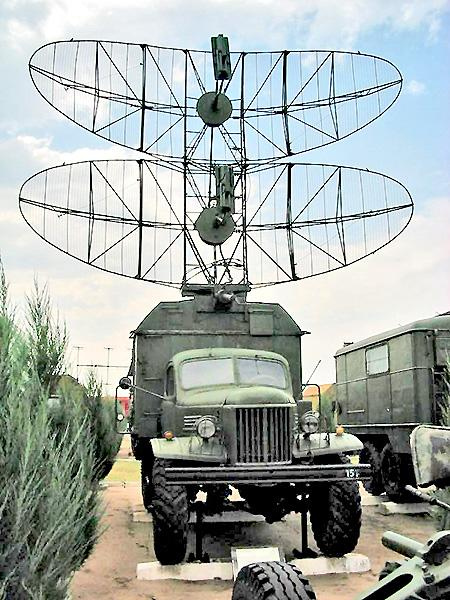
\includegraphics[scale=0.5]{Bekaa_1/FQ2CUDJPd6M.jpg}
	%	\label{fig:scipion} % Unique label used for referencing the figure in-text\end{document}
	%	%\addcontentsline{toc}{figure}{Figure \ref{fig:placeholder}} % Uncomment to add the figure to the table of contents%----------------------------------------------------------------------------------------
	\caption{РЛС П-15, рабочая лошадка сирийских РТВ}%	CHAPTER 2
\end{figure}

Некоторый эффект имели станции РЭП Р-386 (“Терек”) и Р-381 (“Таран”) - несмотря на то, что израильские источники часто пишут о том, что связь самолетов с КП обладала высокой помехозащищенностью, летчики часто говорили об обратном. Особенно много проблем “глушилки” создавала “Фантомам” и “Скайхоком” второй и третьей ударных групп, но об этом мы поговорим позже. Вообще, сирийцы конкретно так пытались подавить каналы наведения истребителей с Е-2 и земли - повторюсь, некоторый эффект от этих действий был.

Вообще, в части аппаратуры была та ещё сборная солянка, что при не самой высокой квалификации конечных пользователей и некотором бардаке с восточным колоритом сводила конечный эффект к нулю.

Что касается непосредственно зенитно-ракетных дивизионов, тот тут ситуация подобная. Экспортные “Квадраты” первых модификаций, С-75, С-125. Все эти комплексы были прекрасно знакомы израильтянам, захватывались ими (по частям и целиком) и ничего нового для них не представляли. Израильтяне отлично знали их возможности, уязвимости, частоты работы и так далее.

Израильская же техника для сирийцев была “терра инкогнита” - они до последнего момента вообще не понимали, с чем вообще столкнутся. Здесь должны были помочь советники - но они, скорее всего, тоже слабо представляли возможности противника.

Пожалуй, наихудшая ситуация для сирийцев сложилась в части самолетов - почти сотне новых F-15 и F-16 они могли противопоставить одну (!) эскадрилью МиГ-23МС (крайне слабый самолет с ужасным БРЭО, большими лапками и небольшой полезностью) и МФ (уже чуть лучше, но до F-16 и МЛД ещё далеко). Плюс все эти модификации были экспортными - с понятно урезанными возможностями БРЭО. Понятно, что большинство из них в бою представляли собой потенциальную мишень.

Основу истребительной авиации сирийцев составляли … все те же МиГ-21 различных модификаций, в основном МФ. В 73-м году это был хороший самолет. В 82-м он безнадежно устарел и часто переходил в разряд вышеупомянутой пилотируемой мишени.

Но самым главным недостатком сирийских вооруженных сил было другое. В отличие от израильтян, у них не было той самой системы, интеграции платформ между собой. Каждый дивизион воевал сам по себе. Связь между батареями отсутствовала. Общее представление об обстановке было утрачено практически сразу после начала операции.

По идее, в решении и этой проблемы должны были помочь советники, в огромных количествах направленные в братскую арабскую республику. По идее, если бы им удалось наладить сопряжение комплексов, выстроить взаимодействие между дивизионами, заставить наконец арабов маневрировать, как им это неплохо удавалось в 73-м году, донести до них угрозу дронов … все могло сложиться и не так плохо.

У меня есть только одно объяснение на этот счет. Большинство в контингенте советников в частях ПВО составляли выходцы из войск ПВО СССР, при этом работать они были вынуждены в основном с комплексами ПВО армии, а это несколько другая истории и другая “философия” ведения войны. Ну и плюс советские ветераны практически открытым текстом говорили, что множество советников были не самыми грамотными, а самыми политически надежными. Ну и это не удивительно …

Подводя итог - сирийские вооруженные силы были оснащены по последнему слову советской экспортной техники, с весьма посредственными характеристиками и крайне паршивой помехозащищенностью. Сирийцы, в отличие от израильтян, сковывали инициативу "на местах" и даже близко не имели сложившейся в ВВС Земли обетованной культуры открытости и признания ошибок. Зато очень любили очковтирательство. 


Ссылка на оригинал \url{https://vk.com/wall-162479647_24239}

К оглавлению на странице \pageref{tablecont}